\subsubsection{\stid{5.01} Software Development Kits} \label{subsubsect:ecosystem-sdk}

\paragraph{Overview} The ST Software Development Kit (SDK) project supports a set of activities focused on 
\begin{itemize}
\item establishing Community Policies aimed at increasing the interoperability between and sustainability of ST software packages, using the xSDK~\cite{xsdk:homepage} community package and installation policies~\cite{xsdk-policies:homepage} as a model.
\item coordinating the delivery of ECP ST products through the Extreme-Scale Scientific Software Stack (E4S)~\cite{e4s:homepage}, a comprehensive and coherent set of software tools, to all interested stakeholders on behalf of ECP ST, including ECP applications and the broader open source community.
\end{itemize}

An ECP ST SDK is a collection of related software products (called packages) where coordination across package teams will improve usability and practices and foster community growth among teams that develop similar and complementary capabilities.  SDKs have the following attributes:
\begin{itemize}
\item Domain scope: Collection makes functional sense.
\item Interaction model: How packages interact; compatible, complementary, interoperable.
\item Community policies: Value statements; serve as criteria for membership.
\item Community interaction: Communication between teams. Bridge culture. Common vocabulary.
\item Meta-infrastructure: Encapsulates, invokes build of all packages (Spack), shared test suites.
\item Coordinated plans: Inter-package planning. Does not replace autonomous package planning.
\item Community outreach: Coordinated, combined tutorials, documentation, best practices.
\end{itemize}

The SDK project is needed within ECP because it will make it simpler for ECP applications to access required software dependencies on ECP target platforms and drastically lower the cost of exploring the use of additional ECP ST software that may be of benefit. In addition, the SDK effort will decrease the ECP software support burden at the major computing facilities by ensuring the general compatibility of ST packages within a single software environment, providing tool support for the installation of ST packages on Facility machines, communicating common requirements for ST software and facilitating the set up of CI testing at the Facilities. This project works closely with the HI 2.4.4 \textit{Deployment of Software at the Facilities} project.

\paragraph{Key  Challenges}
ST software packages have been developed in a variety of very different cultures and are at significantly different levels of software engineering maturity and sophistication. The experience of some of the SDK staff during the formation of the xSDK showed that in this situation, it is challenging to establish common terminology and effective communication, and these are prerequisites to community policies and a robust software release.

Deciding exactly how to deploy the SDKs at the Facilities is itself a challenge. ECP applications will use different combinations of ST software in different configurations. For example, applications will want mathematical libraries capabilities from the xSDK build on top of both MPICH and OpenMPI, and will want different configurations of those mathematical libraries.

\paragraph{Solution Strategy}
The SDK solution strategy involves pursuing interoperability and sustainability goals by grouping ST software projects into logical collections whose members will benefit from a common set of community policies as well as increased communication between members to standardize approaches where sensible and establish better software practices. 

The SDK effort will also facilitate the use of common infrastructure, such as CI testing at the major computing Facilities and the Spack~\cite{gamblin+:sc15} package manager. SDK release and delivery goals will benefit from common package manager and testing infrastructure, including the E4S initiative to provide prebuilt binaries for a variety of architectures.

Recognizing the release readiness and broader maturity differences between ECP ST products, the early release strategy has been to include only those products ready for a joint release in the E4S releases, but to also continue to work with other products in preparing for subsequent release opportunities.

\paragraph{Recent Progress}

E4S release 1.0 was announced in November 2019 on the external E4S website~\cite{e4s:homepage}. The release supports 50 ST products under Linux x86\_64. In February 2020, E4S release 1.1 extended support to both NVIDIA and AMD GPUs with the inclusion of CUDA and ROCm in a single image under Linux x86\_64. Release 1.1 also introduced support for the Linux ppc64le platform that supports CUDA 10.1. E4S releases contain HPC as well as AI/ML software including TensorFlow and PyTorch. The E4S DocPortal, accessible from the E4S website, was created to rake information from E4S product GitHub pages and provide it in a single location with the most up-to-date information about releases, installation instructions, etc. The E4S validation testsuite~\cite{e4s:validation} was introduced with support for LLVM and other ST products.

In October 2020, E4S v1.2 included an x86\_64 image with 67 E4S products. E4S images are now available for download on DockerHub under the ecpe4s area for testing and will be released on the E4S website in November 2020. The E4S Spack Build Cache now includes binaries for ppc64le as well as x86\_64 and includes over 22,000 total binaries. E4S containers now support custom images for ECP applications such as WDMapp and Pantheon (see Figure~\ref{fig:SpackBuildCacheWDMapp}). The E4S build cache has improved the the build times for these codes significantly. 
\begin{figure}
        \centering
        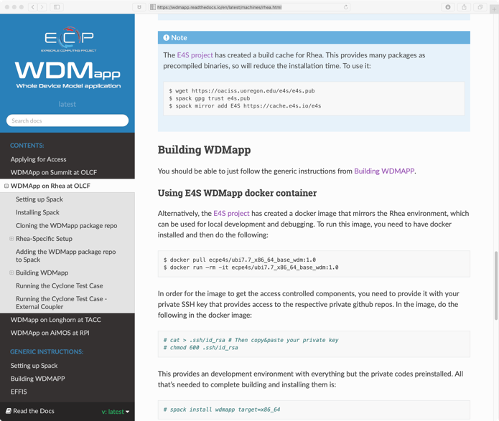
\includegraphics[width=0.9\linewidth]{projects/2.3.5-Ecosystem/2.3.5.01-Ecosystem-SDK/SpackBuildCacheWDMapp}
        \caption{WDMapp documentation for how to use the E4S WDMapp Docker container to speed up WDMapp installation by leveraging the E4S Spack build cache.}
        \label{fig:SpackBuildCacheWDMapp}
\end{figure}

Also in October 2020, Version 1 of the E4S Community Policies was announced~\cite{e4s:policies}. The E4S Community Policies will serve as membership criteria for E4S member packages. The E4S Community Policies have their genesis in the xSDK Community Policies, and have a similar purpose. Their purpose is to help address sustainability and interoperability challenges within the complex software ecosystem that ECP ST is a part of.

The process of establishing Version 1 of the E4S Community Policies was a multi-year effort led by the ECP SDK team, including representation from Programming Models and Runtimes, Development Tools, Math Libraries, Data and Vis, and Software Ecosystem and Delivery. This team reviewed the existing xSDK Community Policies and selected those policies that were most generally applicable to all of ECP ST, and not specific to math libraries. From there, the chosen policies were refined and gaps were analyzed.

An early draft was presented to ECP ST leadership, after which an updated draft was socialized with all of ECP ST. The feedback gathered was incorporated into another draft that was again shared broadly across ECP ST. Feedback examples can be seen in Figure~\ref{fig:e4s-policy-feedback}. After considering the latest feedback, the first version of the policies was finalized. A strong effort was made to involve all interested community members and seriously consider the feedback received.

\begin{figure}
        \centering
        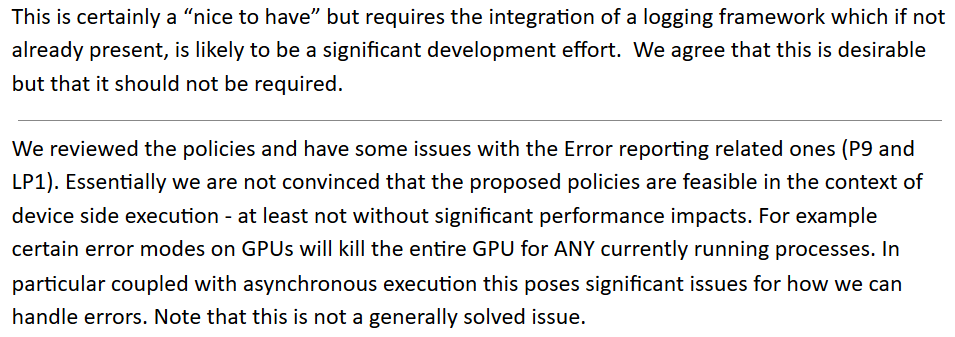
\includegraphics[width=0.9\linewidth]{projects/2.3.5-Ecosystem/2.3.5.01-Ecosystem-SDK/E4S-policy-comment}
        \caption{Two examples of policy feedback received from the ECP ST development community. Comments commonly touched on issues such as appropriateness, both broadly and to specific types of software found within ST, as well as clarity and feasibility.}
        \label{fig:e4s-policy-feedback}
\end{figure}

In addition to the policies shown in Figure~\ref{fig:E4S-Community-Policies-V1} a second list of Future Revision policies was also created. These policies are not currently E4S membership criteria, but will be very seriously considered in future versions. In most cases, these policies require further refinement or planning prior to adoption. The topics that these policies address provide information about likely subject areas for E4S policies going forward and are critical to ongoing communication with the E4S community.

%In January 2019, E4S Release 0.2 was posted to the new external E4S website~\cite{e4s:homepage}. It includes a subset of ECP ST software products, and demonstrates the target approach for future delivery of the full ECP ST software stack. Also available are a number of ECP ST software products that support a Spack package, but are not yet fully interoperable. As the primary purpose of the 0.2 release is demonstrating the ST software stack release approach, not all ECP ST software products were targeted for this release. Software products were targeted primarily based on existing Spack package maturity, location within the scientific software stack, and ECP SDK developer experience with the software.

%E4S release 0.2 is also available through a container release that includes support for Docker, Singularity, Shifter, and Charliecloud. The release allows ECP applications that use MPI to be released in a binary form using libraries from the container. The MPI runtime layer can be substituted during execution with the native MPI (e.g., Intel MPI, Cray MPICH, MVAPICH2) that uses the high-speed inter-node network interconnect.

%The initial set of ECP ST SDKs was finalized in December 2018 after consultation with ECP ST leadership. The make up of the SDKs is expected to evolve over time, but the current definitions provide a basis for beginning to form the associated SDK communities. Figure~\ref{fig:sdk-definition1} illustrates the initial division of ST products into SDKs. Note that the ecosystem group listed is currently not anticipated to become a SDK. Rather, the members of that group will be considered E4S software not associated with a specific SDK and will be responsible only for the general community policies that will apply to all ECP ST products. This is due to the large variety of software included in that group and an anticipated lack of commonality that will lead to additional beneficial community policies. Smaller-scale collaboration between these teams may be encouraged in select cases.

%\begin{figure}[htb]
%        \centering
%        \includegraphics[width=6.5in]{projects/2.3.5-Ecosystem/2.3.5.01-Ecosystem-SDK/SDKdefinition1}
%        \caption{\label{fig:sdk-definition1}The above graphic shows the breakdown of ECP ST products into 6 SDKs ( the first six columns).  The rightmost column lists products that are not part of an SDK, but are part of Ecosystem group that will also be delivered as part of E4S. The colors denoted in the key map all of the ST products to the ST technical area they are part of.  For example, the xSDK consists of products that are in the Math Libraries Technical area, plus TuckerMPI which is in the Ecosystem and Delivery technical area.}
%\end{figure}

\paragraph{Next Steps}
Current and near-term efforts include:

\begin{itemize}
\item  Defining a process for documenting and verifying compatibility with E4S Community Policies.
\item  Assisting with E4S deployment to computing Facilities.
\item  Adding additional ST software to E4S.
\item  Assisting with establishing workflows around the maintenance of multi-package CI builds at computing facilities.
\item  Starting work on Version 2 of the E4S Community Policies.
\item  Supporting SDK-specific efforts focused on the needs of each SDK, with a particular emphasis on sustainability.
\end{itemize}

